\documentclass{beamer}

\usepackage[utf8]{inputenc}
\usepackage{graphicx}
\usepackage{default}

\begin{document}
  \begin{frame}
    \frametitle{Introduction}
    Notre problème est de connaître le meilleur moyen pour chauffer rapidement une piscine. Pour cela, nous allons calculer les apports et pertes thermiques dans plusieurs cas, avant de les comparer. Nous étudierons tout d’abord le cas de la piscine seule. Ensuite, nous nous intéresserons aux cas où l’on couvre la piscine avec une bâche, puis deux bâches.
    %Content goes here
  \end{frame}
  \begin{frame}
   \frametitle{Hypothèses}
   \begin{enumerate}
    \item Parois de la piscine sont parfaitement isolées
    \item Fond de la piscine foncé
    \item Pertes thermiques par rayonnement négligeables
    \item Résistance thermique de la bâche
    \item Surface de l’eau solide d’épaisseur nulle
   \end{enumerate}



 






  \end{frame}
  \begin{frame}
   \frametitle{schema}
   \begin{figure}[ht!]
    \centering
    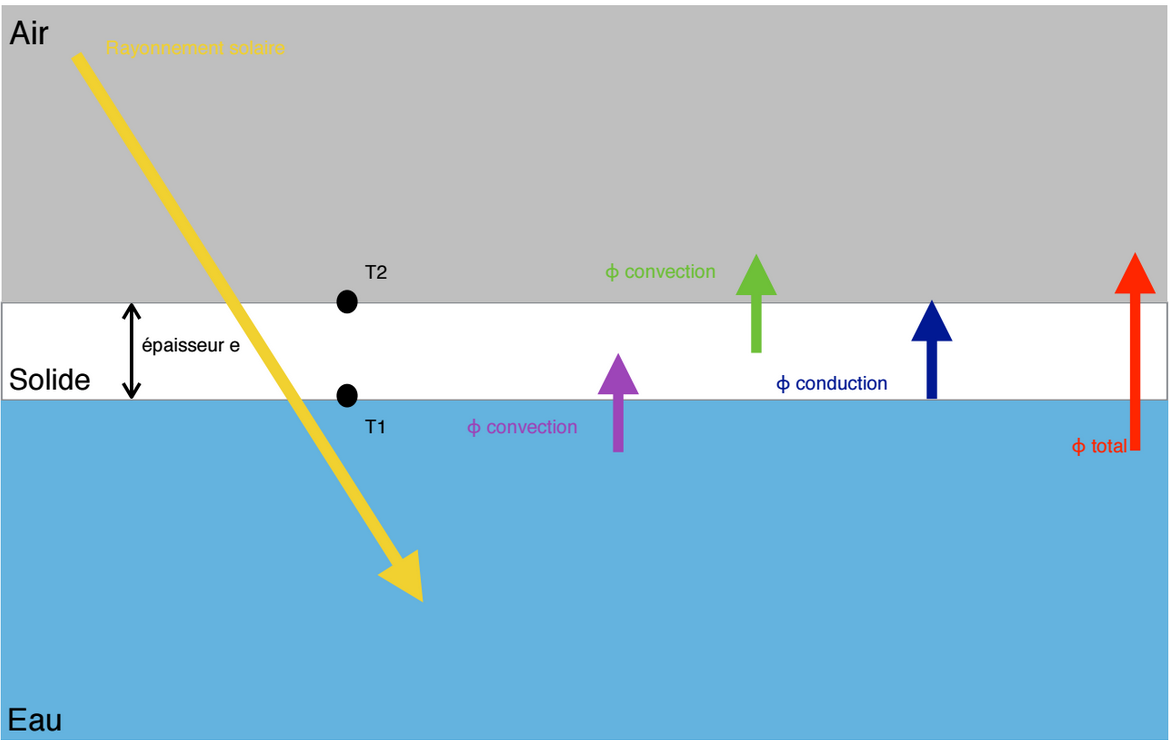
\includegraphics[width=90mm]{thermo.png}
    \caption{Mod\'{e}lisation du cas g\'{e}n\'{e}ral \label{overflow}}
   \end{figure}
  \end{frame}

  \begin{frame}
    \[h_{eau}*S*(T_{eau} - T_{1}) = \phi_{convection(e->s}\]
    \[\frac{\lambda}{e} * S * (T_{1} - T_{2}) = \phi_{conduction}\]
    \[h_{air}*S*(T_{2} - T_{air}) = \phi_{convection(s->air)}\]
    %More content goes here
  \end{frame}
  \begin{frame}
    \[T_{eau} - T_{air} = T_{eau} - T_{1} + T_{1} - T_{2} - T_{air}\]
    \[T_{eau} - T_{air} = \frac{\phi_{convection(e->s)}}{h_{eau}*S} + \frac{\phi_{conduction}}{\frac{\lambda}{e} * S} + \frac{\phi_{convection(s->air)}}{h_{air}*S} \]
    \[T_{eau} - T_{air} = \phi_{tot}(\frac{1}{h_{eau}*S} + \frac{1}{\frac{\lambda}{e} * S} + \frac{1}{h_{air}*S}) \]
    \[\phi_{tot} = \frac{T_{eau} - T_{air}}{\frac{1}{S}(\frac{1}{h_{eau}} + \frac{e}{\lambda} + \frac{1}{h_{air}})}\]
    %Content goes here
  \end{frame}
  \begin{frame}
   \frametitle{Coefficient de conductivité thermique}
   On considère que l'air transmet la chaleur par conduction pour simplifier les calculs.
   Les plastiques et l'air sont en série.
   \[R_{bache} = R_{e} + 2 * R_{p}\]
   \[R_{bache} = \frac{e_{a}}{\lambda_{a} * S} + 2 * \frac{e_{p}}{\lambda_{p} * S}\]
   \[R_{bache} = \frac{e}{\lambda * S}\]
   \[\lambda_{bache} = \frac{e}{R_{bache} * S} = \frac{e}{S* \frac{e_{a}}{\lambda_{a} * S} + 2 * \frac{e_{p}}{\lambda_{p} * S}}\]
   
  \end{frame}

  \begin{frame}
   \frametitle{Choix du codage en Python}
   Le flux dépend de la température et la température dépend du flux, comment faire ?
Nous avons écrit un programme en python qui répète:
    \begin{enumerate}
     \item Calculer le flux à partir de la température
     \item Faire varier la température en soumettant l’eau au flux pendant une seconde

    \end{enumerate}

  \end{frame}
  \begin{frame}
   \frametitle{Sans bache sans vent}
   
  \end{frame}


% etc
\end{document}
